% !TEX TS-program = pdflatex
% !TEX encoding = UTF-8 Unicode
%%
%% This is file `sample-sigconf.tex',
%% generated with the docstrip utility.
%%
%% The original source files were:
%%
%% samples.dtx  (with options: `sigconf')
%% 
%% IMPORTANT NOTICE:
%% 
%% For the copyright see the source file.
%% 
%% Any modified versions of this file must be renamed
%% with new filenames distinct from sample-sigconf.tex.
%% 
%% For distribution of the original source see the terms
%% for copying and modification in the file samples.dtx.
%% 
%% This generated file may be distributed as long as the
%% original source files, as listed above, are part of the
%% same distribution. (The sources need not necessarily be
%% in the same archive or directory.)
%%
%%
%% Commands for TeXCount
%TC:macro \cite [option:text,text]
%TC:macro \citep [option:text,text]
%TC:macro \citet [option:text,text]
%TC:envir table 0 1
%TC:envir table* 0 1
%TC:envir tabular [ignore] word
%TC:envir displaymath 0 word
%TC:envir math 0 word
%TC:envir comment 0 0
%%
%%
%% The first command in your LaTeX source must be the \documentclass command.
\documentclass[sigconf]{acmart}

\settopmatter{printacmref=false} % Removes citation information below abstract
\renewcommand\footnotetextcopyrightpermission[1]{} % removes footnote with conference information in first column
%%\pagestyle{plain} % removes running headers
\thispagestyle{empty}
%%
%% \BibTeX command to typeset BibTeX logo in the docs
\AtBeginDocument{%
  \providecommand\BibTeX{{%
    \normalfont B\kern-0.5em{\scshape i\kern-0.25em b}\kern-0.8em\TeX}}}

%% Rights management information.  This information is sent to you
%% when you complete the rights form.  These commands have SAMPLE
%% values in them; it is your responsibility as an author to replace
%% the commands and values with those provided to you when you
%% complete the rights form.
\setcopyright{none}
\copyrightyear{}
\acmYear{}
\acmDOI{}

%% These commands are for a PROCEEDINGS abstract or paper.
\acmConference[]{}{}{}
\acmBooktitle{BDM Socio - Technical Optimizer}
\acmPrice{}
\acmISBN{}


%%
%% Submission ID.
%% Use this when submitting an article to a sponsored event. You'll
%% receive a unique submission ID from the organizers
%% of the event, and this ID should be used as the parameter to this command.
%%\acmSubmissionID{123-A56-BU3}

%%
%% The majority of ACM publications use numbered citations and
%% references.  The command \citestyle{authoryear} switches to the
%% "author year" style.
%%
%% If you are preparing content for an event
%% sponsored by ACM SIGGRAPH, you must use the "author year" style of
%% citations and references.
%% Uncommenting
%% the next command will enable that style.
%%\citestyle{acmauthoryear}

%%
%% end of the preamble, start of the body of the document source.
\begin{document}

%%
%% The "title" command has an optional parameter,
%% allowing the author to define a "short title" to be used in page headers.
\title{BDM Socio - Technical Optimizer}


%%
%% The "author" command and its associated commands are used to define
%% the authors and their affiliations.
%% Of note is the shared affiliation of the first two authors, and the
%% "authornote" and "authornotemark" commands
%% used to denote shared contribution to the research.
\author{Boi Biagio}
\email{b.boi@studenti.unisa.it}
\affiliation{%
  \institution{Universit\'a degli studi di Salerno}
  \streetaddress{}
  \city{Salerno}
  \state{}
  \country{Italy}
  \postcode{}
}

\author{Silvio Di Martino}
\email{s.dimartino21@studenti.unisa.it}
\affiliation{%
  \institution{Universit\'a degli studi di Salerno}
  \streetaddress{}
  \city{Salerno}
  \state{}
  \country{Italy}
  \postcode{}
}

\author{Gerardo Martino}
\email{g.martino11@studenti.unisa.it}
\affiliation{%
  \institution{Universit\'a degli studi di Salerno}
  \streetaddress{}
  \city{Salerno}
  \state{}
  \country{Italy}
  \postcode{}
}

%%
%% By default, the full list of authors will be used in the page
%% headers. Often, this list is too long, and will overlap
%% other information printed in the page headers. This command allows
%% the author to define a more concise list
%% of authors' names for this purpose.
\renewcommand{\shortauthors}{}

%%
%% The abstract is a short summary of the work to be presented in the
%% article.
\begin{abstract}
Recent studies have proven that software development is a social activity, in fact it is possible to measure the level of coordination between developers and the organization in order to improve the quality of software product in various respects. Software Products are constantly evolving, so maintenance activities play a crucial role in enabling you to have a useful product. With the support of tools and Refactoring technique, we can improve the source code automatically, but one of the relevant key factor that at moment these software do not perform is how we can improve the social-technical aspect, meaning improve a restructuring of the developer community and team rearrangement to improve a software product. The study starts with a repository mining activity, and then builds the graphs useful to represent the communication among developers (dev-dev), the collaboration among developers (dev-file) and the dependencies among files (file-file). After that by using the Genetic Algorithms we have processed the information collected in order to optimize the relationships between the members of the team \cite{palomba1}.
\end{abstract}

%%
%% Keywords. The author(s) should pick words that accurately describe
%% the work being presented. Separate the keywords with commas.
\keywords{mining, optimization, refactoring, genetic algorithms}

%% A "teaser" image appears between the author and affiliation
%% information and the body of the document, and typically spans the
%% page.

\begin{teaserfigure}
\rule{\linewidth}{1mm}
%%  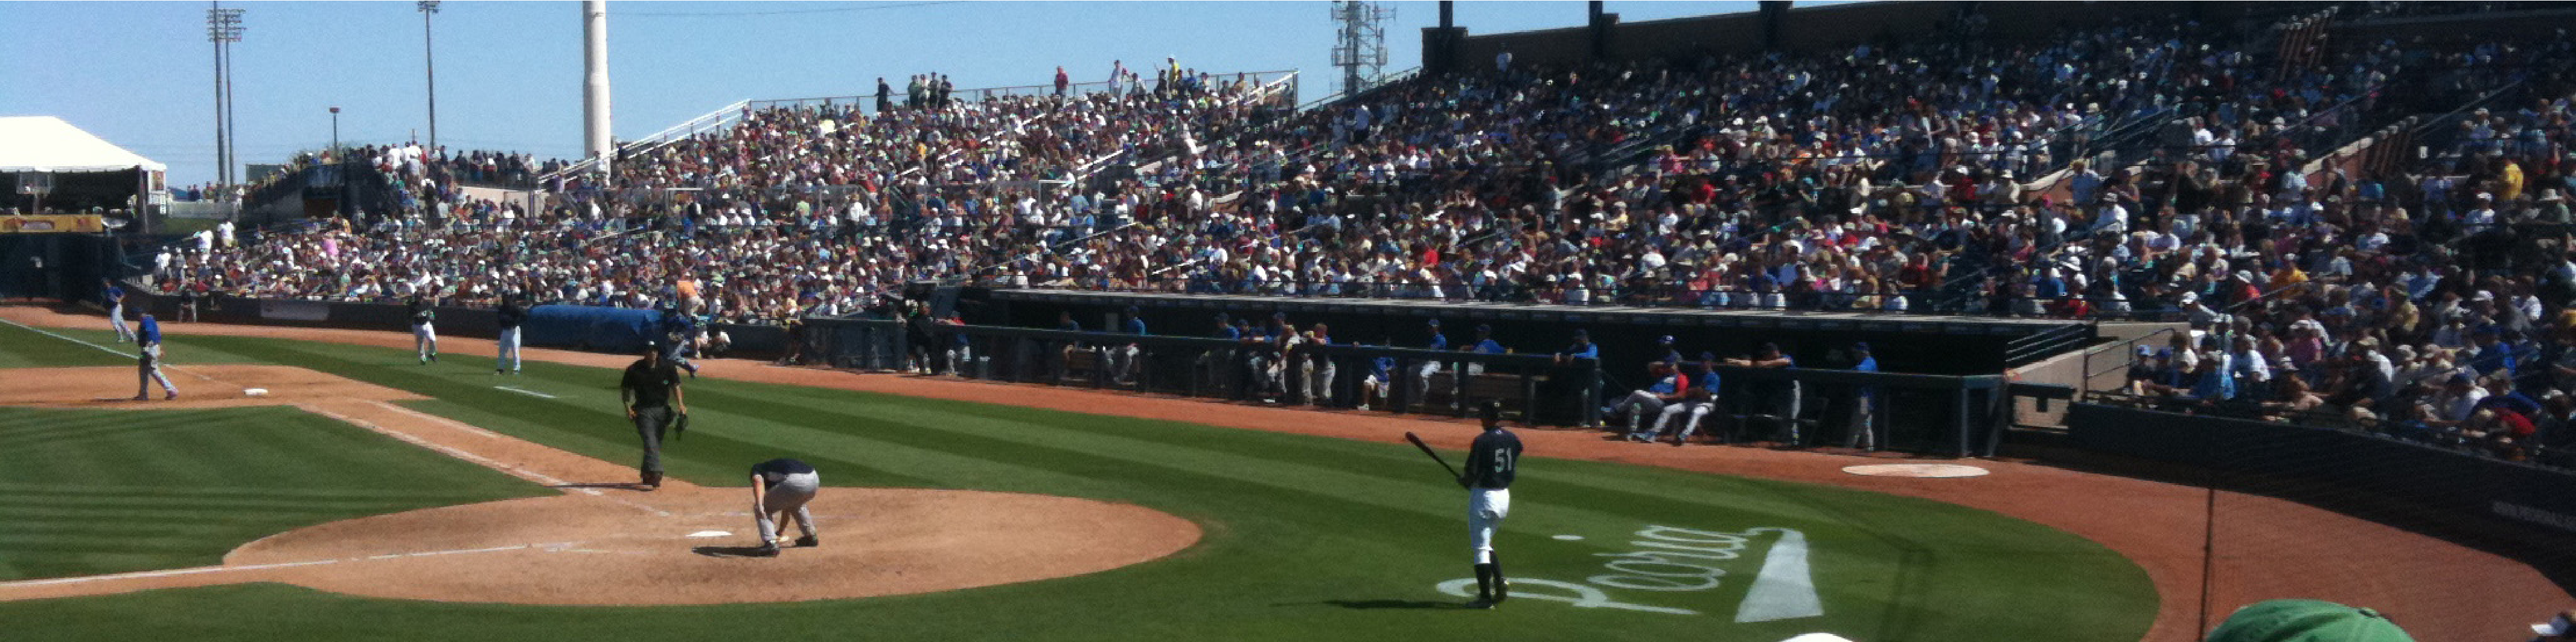
\includegraphics[width=\textwidth]{sampleteaser}
%%  \caption{Insert text here}
%%  \Description{insert description here}
%%  \label{fig:teaser}
\end{teaserfigure}

%%
%% This command processes the author and affiliation and title
%% information and builds the first part of the formatted document.
\maketitle

\section{Introduction}
In detail the first step that we did was searching for tools and libraries to get the necessary information. In particular, to mine the information from communications between developers we used the {\itshape GitHub API }to get data on issues (comments and answers); while regarding information related to commit effettuati from developers on source files, through the framework {\itshape PyDriller} (\url{https://pydriller.readthedocs.io/en/latest/}), we have easily extracted information from any Git repository, such as commits, developers, modifications, diffs, and source codes, and quickly export as CSV file, the mining of information ended with the study of the relationship between files, in particular the structural code dependency analysis was carried out with {\itshape Depends} (\url{https://github.com/multilang-depends/depends.git}), a source code dependency extraction tool, designed to infer syntactical relations among source code entities, such as files and methods, from various programming languages.

The next step was the representation of this information by means of adjacent lists, that through the framework {\itshape NetworkX} (\url{https://networkx.org/}), we have been easily transformed into graphic elements (graphs). Once the three individual graphs have been obtained, they were subsequently merged to have all the communication, collaboration and coupling information represented by one single structure. 

Finally the last step consists of the execution of a Genetic Algorithm (GA) through the framework {\itshape Deap} (\url{https://deap.readthedocs.io/en/master/}), able to find and optimize a version of the starting graph given as input, taking into account the objective functions to be optimised \cite{palomba1}.

\section{Related Work}

\subsection{Dev-Dev Implementation}
To obtain data regarding the developer, methods have been implemented through the APIs made available by GitHub, that allow us to extrapolate various information from the repositories, including the list of developers who contributed to the development and the number of responses of those to the questions.
The extracted output allowed us to build a square matrix, on whose rows and columns the developers find space. The element {\itshape (i, j)} will be an integer representing the number of responses to the same thread between developer i and developer j. Here is an example matrix:

\begin{figure}[h]
  \centering
  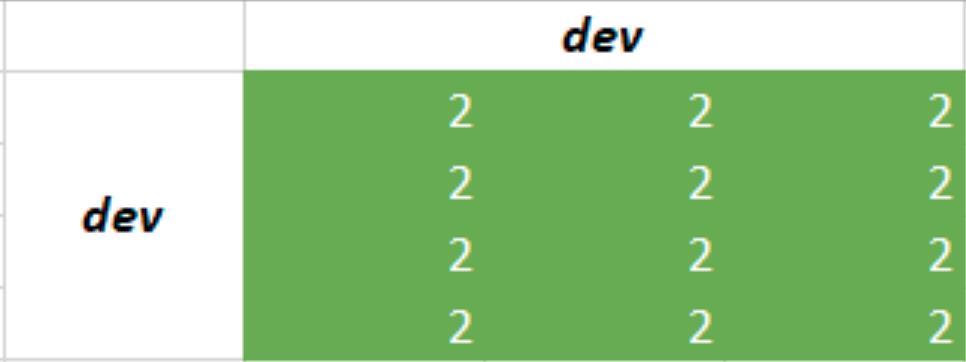
\includegraphics[width=\linewidth]{img_4}
  \caption{Example of Dev-Dev matrix.}
  \Description{}
\end{figure}

After the construction of the above matrix and through the use of the {\itshape NetworkX}, a Python tool for the creation, manipulation, and study of data structures, we obtained an undirected weighted graph in which the nodes represent the developers and the edges the communications among them. Meaning that if a developer participated in at least one issue thread with another developer, an edge is created to connect them. The weights are represented by the total number of replies given in a shared thread over all the threads of the project, without considering the criticality of the issue.

\begin{figure}[h]
  \centering
  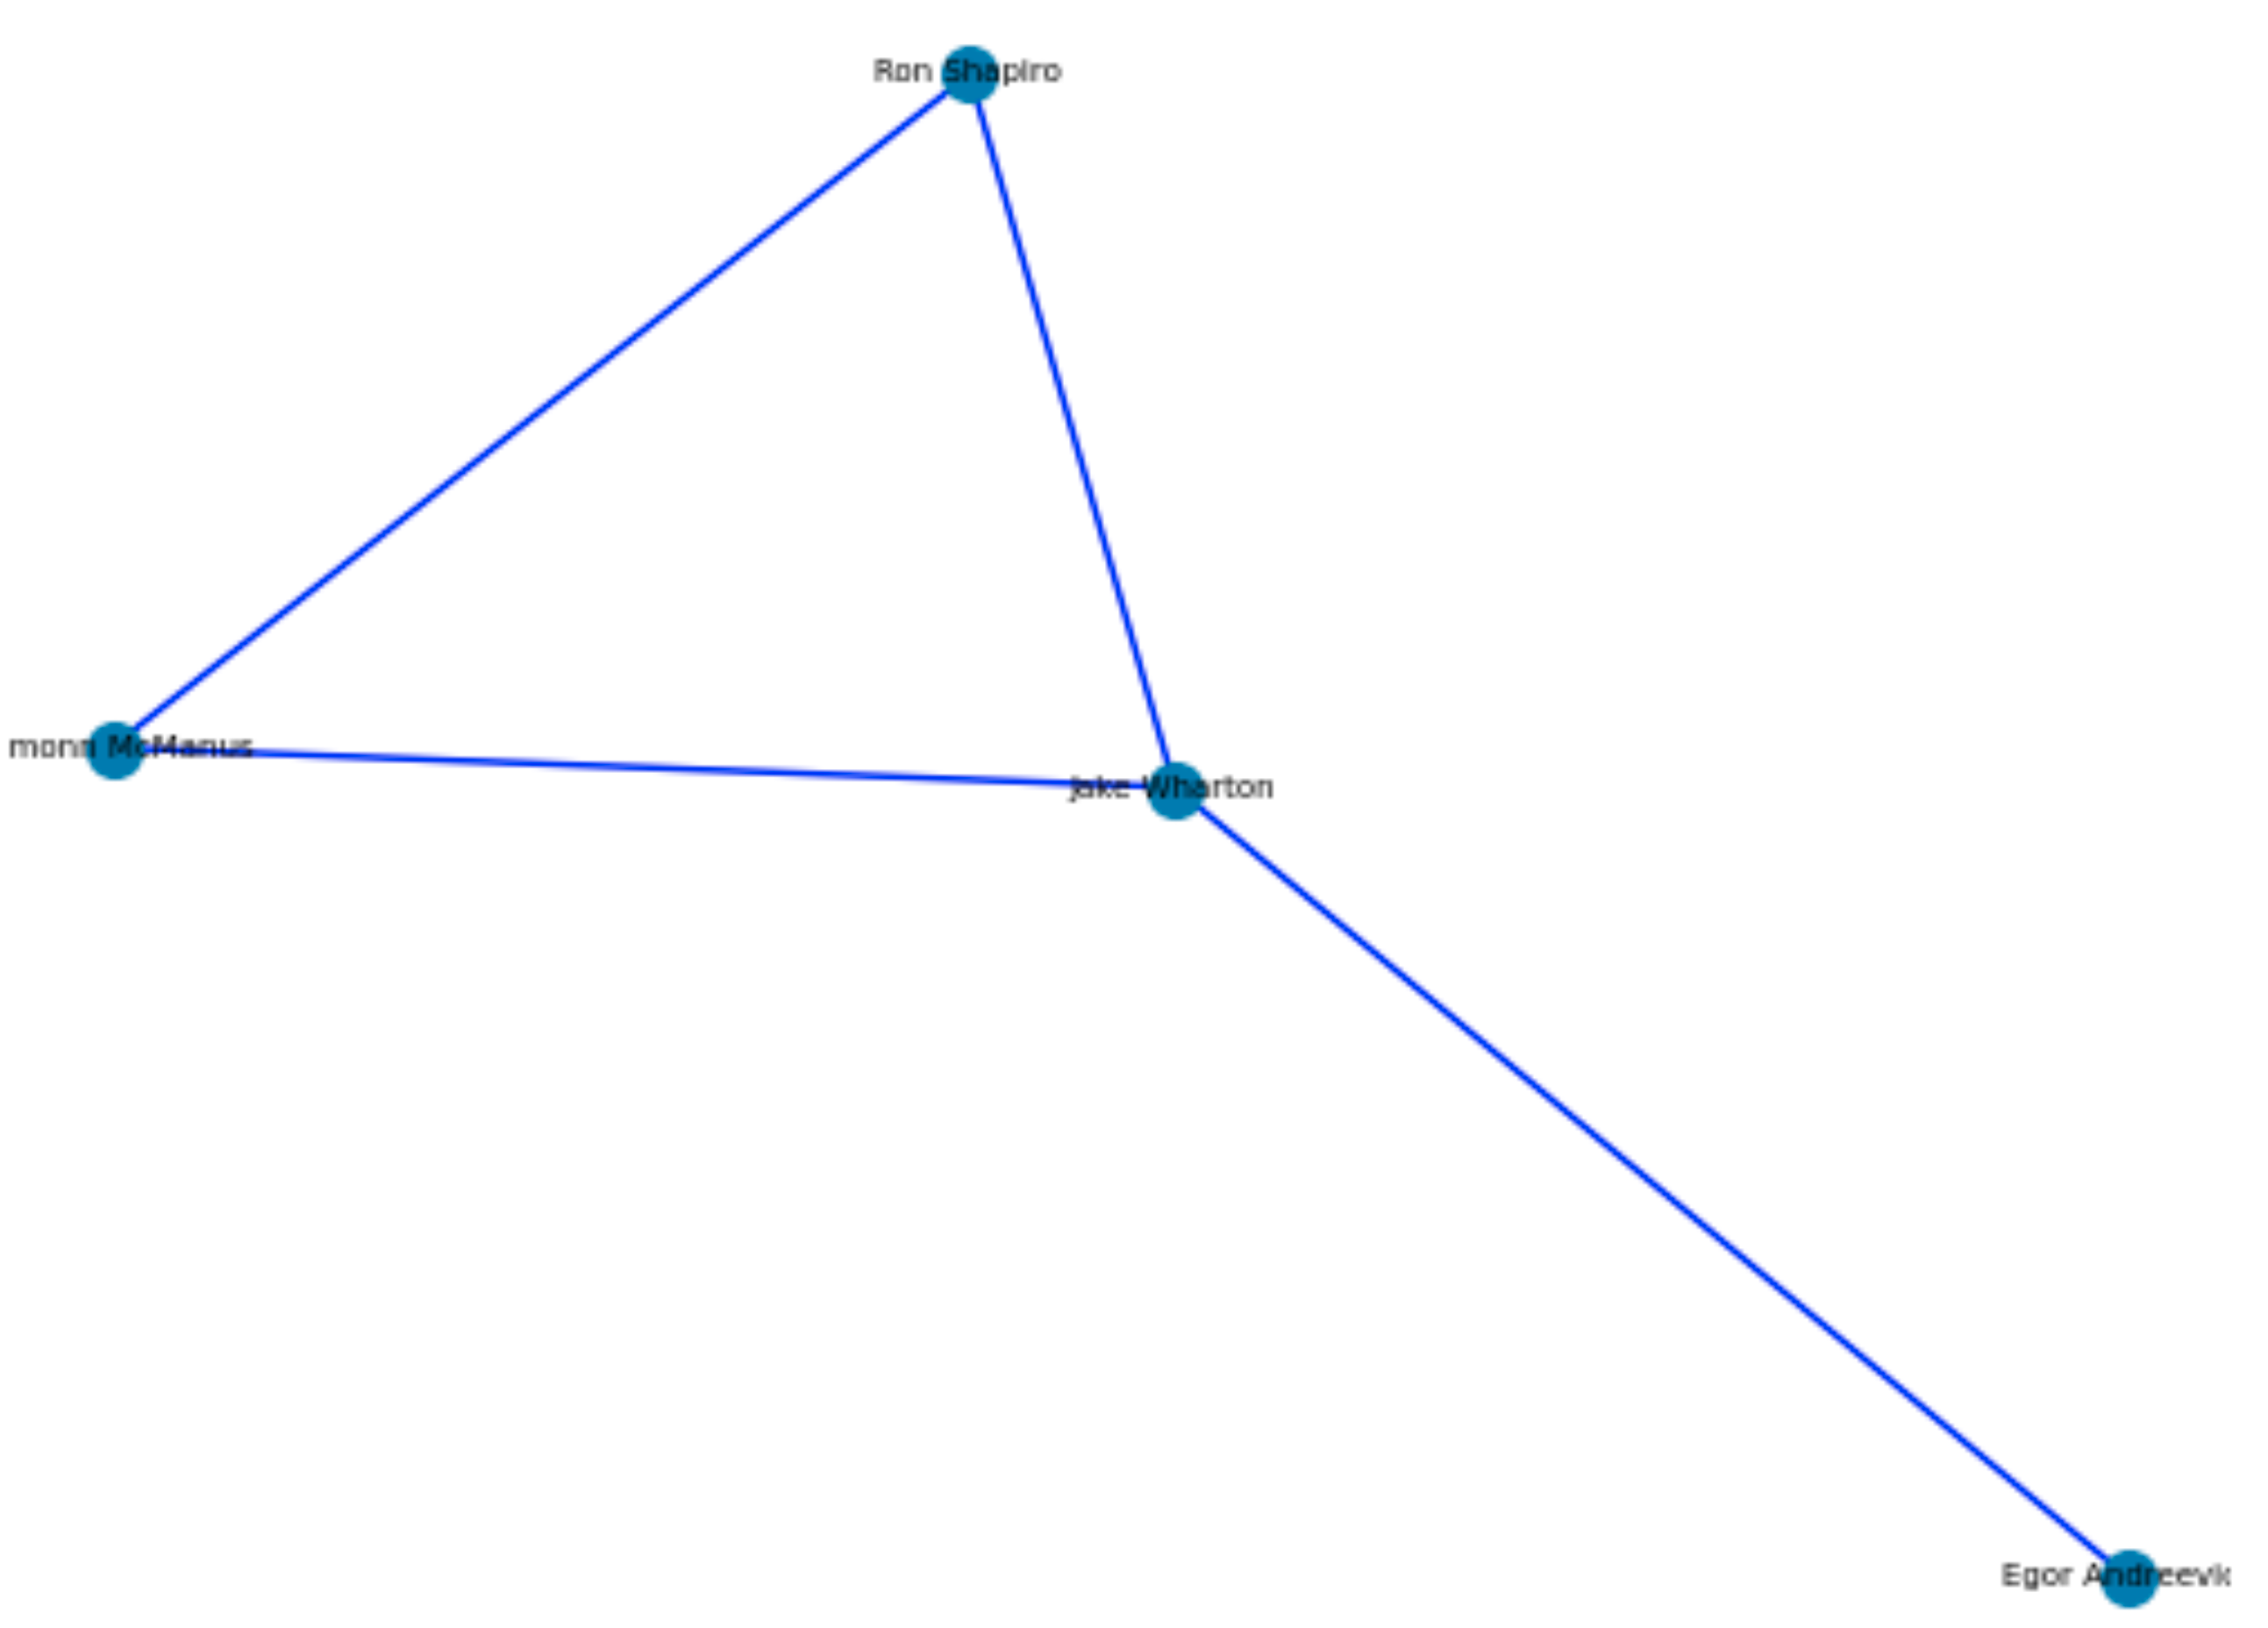
\includegraphics[width=\linewidth]{img_8}
  \caption{dev-dev graph}
  \Description{}
\end{figure}

\subsection{Dev-File Implementation}
Then through the use of the {\itshape PyDriller} library, it was possible to analyze the repository and extrapolate information on the commits. In particular, methods have been implemented to obtain information on the number of commits made by each developer on each file.
Another matrix was then built, on whose rows we find the developers and on whose columns we find the files: element {\itshape (i, j)} will be an integer representing the number of commits that the developer i has made on file j. Here is an example matrix:

\begin{figure}[h]
  \centering
  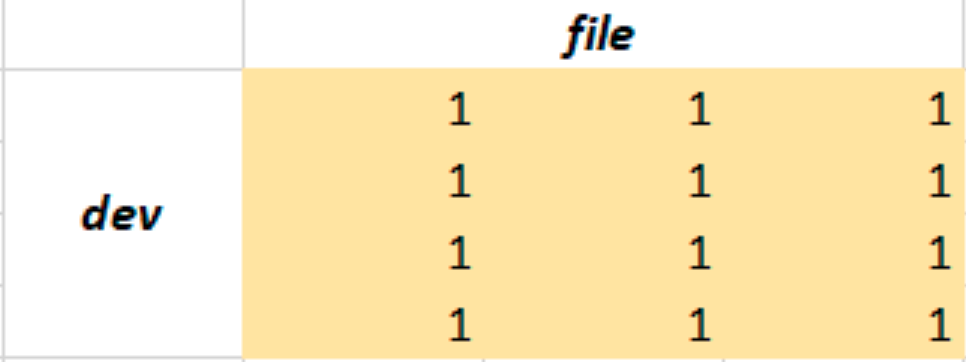
\includegraphics[width=\linewidth]{img_3}
  \caption{Example of Dev-File matrix.}
  \Description{}
\end{figure}

Also in this case, through {\itshape NetworkX} , a bipartite graph has been obtained, as we have only two types of nodes, developer and file, connected. A developer node is connected to a file node if the developer has committed at least once that file. The weight on the edges consists of the developer’s total number of commits on that file in the considered

\begin{figure}[h]
  \centering
  \includegraphics[width=\linewidth]{img_9}
  \caption{dev-file graph}
  \Description{}
\end{figure}

\subsection{File-File Implementation}
Finally, to automate the dependency extraction process we invoked the Depends framework in order to obtain information regarding the dependencies between the various source files.

The framework {\itshape Depends} supports major dependency types, including:
\begin{itemize}
\item {\verb|Call|}: function/method invoke
\item {\verb|Cast|}: type cast
\item {\verb|Contain|}: variable/field definition
\item {\verb|Create|}: create an instance of a certain type
\item {\verb|Extend|}: parent-child relation
\item {\verb|Implement|}: implemented interface
\item {\verb|Import/Include|}: for example, java import, c/c++ import, ruby require
\item {\verb|Parameter|}: as a parameter of a method
\item {\verb|Return|}: returned type
\item {\verb|Throw|}: throw exceptions
\item {\verb|Use|}: use or set variables
\item {\verb|ImplLink|}: the implementation link between call and the implementation of prototype
\end{itemize}



The extracted data led to the construction of a third matrix, on whose rows and columns we find the files: the element {\itshape (i, j)} corresponds to the total number of dependencies between the files {\itshape i} and {\itshape j} (in terms of the sum of the different types of dependencies) as shown in Figure 3.

\begin{figure}[h]
  \centering
  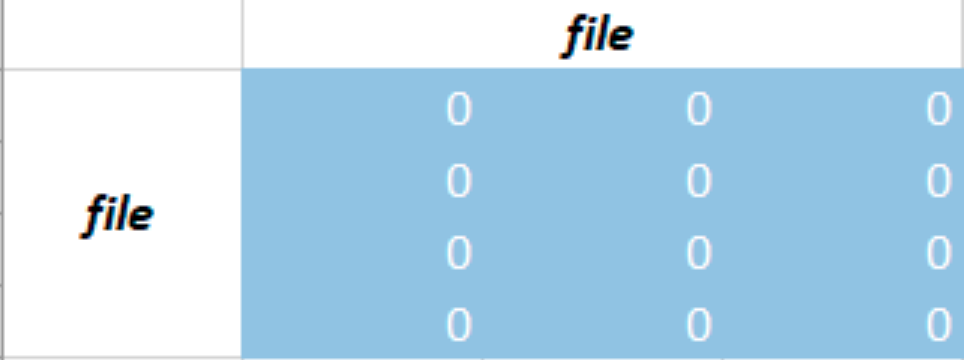
\includegraphics[width=\linewidth]{img_2}
  \caption{Example of File-File  matrix.}
  \Description{}
\end{figure}

Using {\itshape NetworkX}, the file-file graph has been obtained, in which a file node is connected with another if it contains a reference to a code component contained in another file or vice versa. The obtained graph is then undirected, and the weights on the edges represent the actual number of references present among the two source files.

\begin{figure}[h]
  \centering
  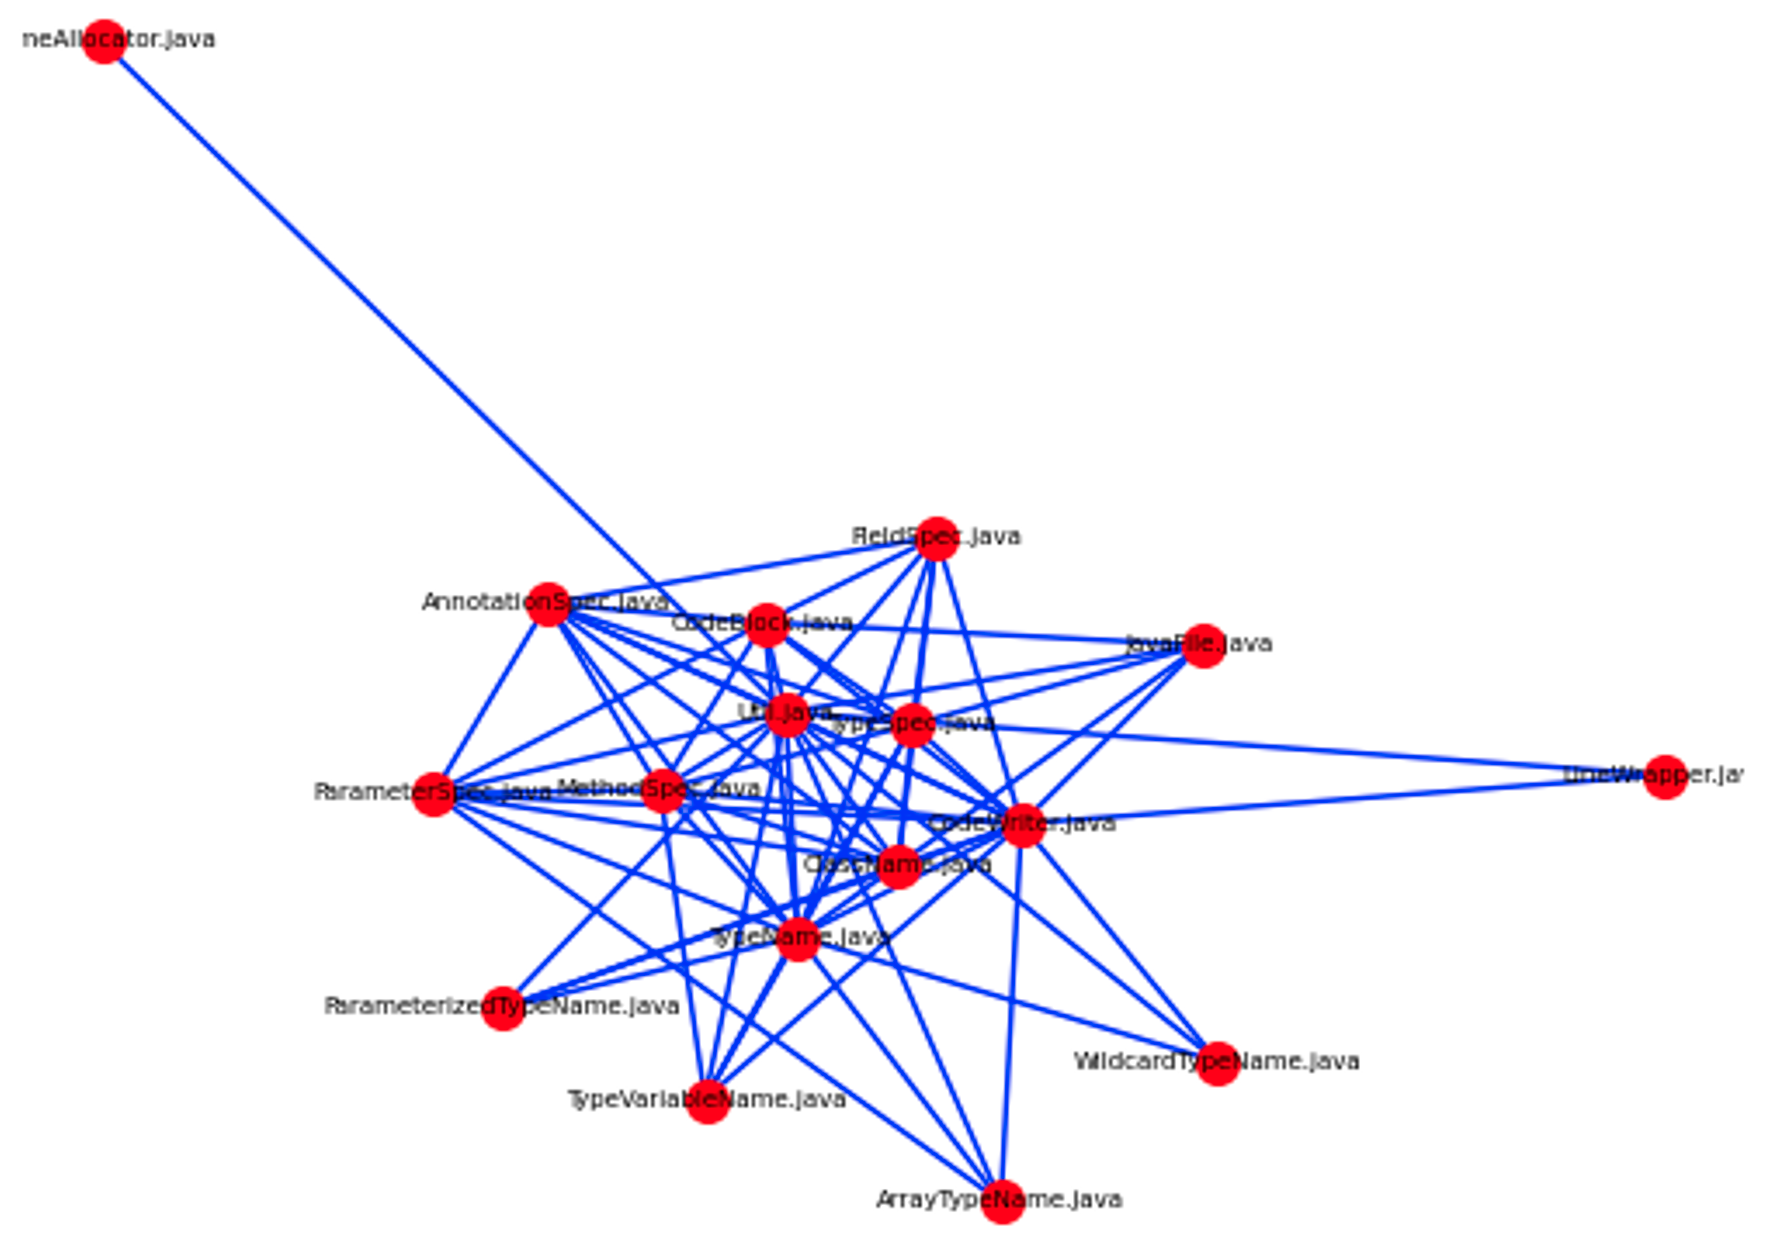
\includegraphics[width=\linewidth]{img_10}
  \caption{file-file graph}
  \Description{}
\end{figure}

At the end of the extraction activity, we proceed with the creation of a single matrix, which consists of a merge of the above 3 matrices obtained.
Below, we show an example of a resulting matrix, obtained by combining the 3 exemplary matrices as shown in Figure 4.

\begin{figure}[h]
  \centering
  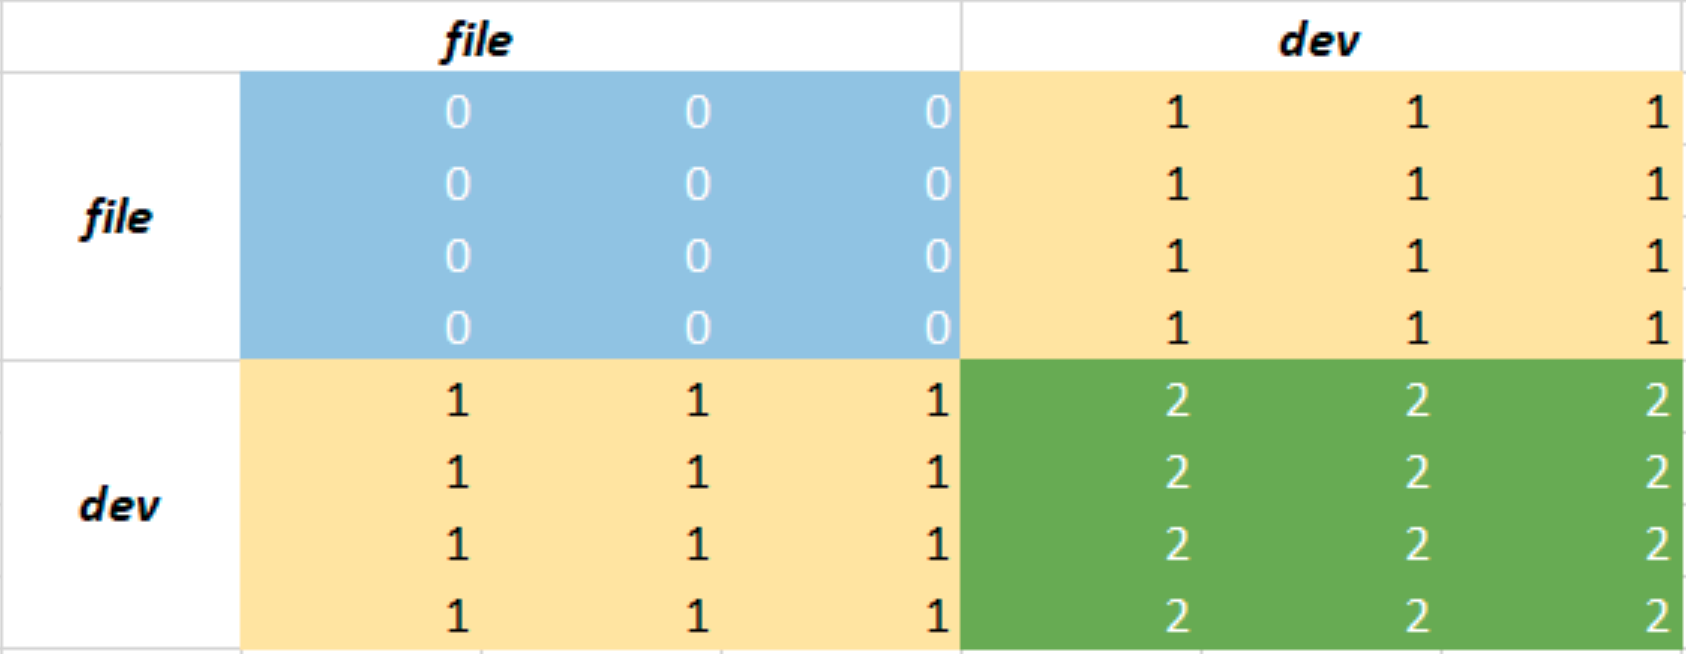
\includegraphics[width=\linewidth]{img_1}
  \caption{Combination of the three matrix}
  \Description{}
\end{figure}

It is necessary to emphasize the fact that in the merge it was necessary to transpose one of the three matrices {\itshape (DEV-FILE --> FILE-DEV) } in order to maintain consistency and coherence in the structure.

\section{Genetic Algorithm Execution}

In this phase we use the framework {\itshape Deap} for rapid prototyping and testing of {\itshape Genetic Algorithm} techniques. So we initialized the population in which each individual is represented by an adjacency matrix that is structured in the same manner of the starting matrix and pseudo-randomly value.

The keypoint is the definition of a multi-objective fitness function: the main goal is \textit{maximizing} the communication and the collaboration between developers, \textit{minimizing} the coupling among components. Besides these three objectives, it is also essential to minimize the changes from the starting graph to the output graph to prevent the GA from excessively altering the original structure while optimizing the objectives. As suggested by Palomba et al. \cite{palomba1}, this equation reports the fitness function, to have a better comprehensibility we refer to different parts of the graph with different names, i.e., $G_{dev-dev}$, $G_{dev-file}$, and $G_{file-file}$.

\begin{figure}[h]
  \centering
  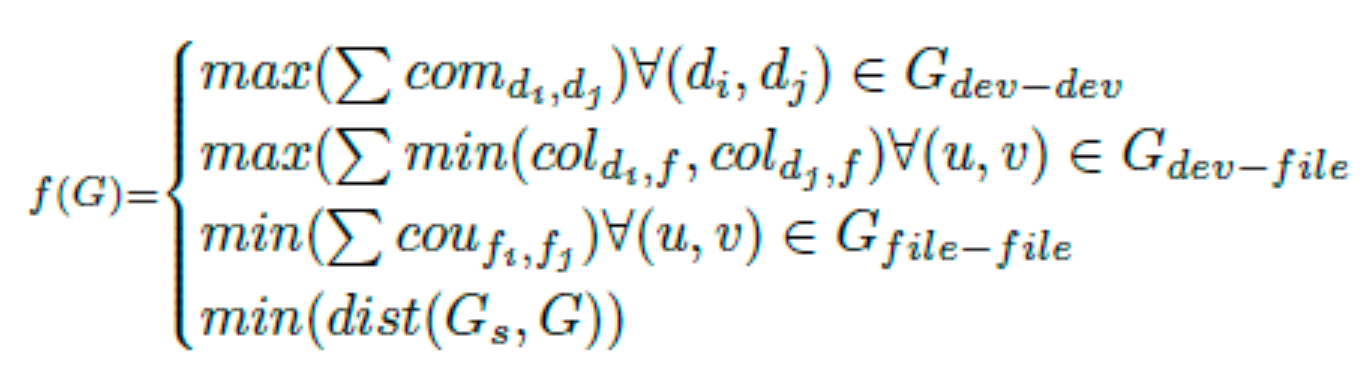
\includegraphics[width=\linewidth]{img_5}
  \Description{}
\end{figure}

where $com_{d_i,d_j}$ is the degree of communication between developers $d_i$ and $d_j$ in the dev-dev graph, max($col_{u_i;v}$; $col_{u_j;v}$) represents the number of co-commits of developers $d_i$ and $d_j$ on the file $f$, $cov_{f_i,f_j}$ is the degree of coupling between files $f_i$ and $f_j$ , and dist($G_s$, G) is the minimum number of operations to transform graph $G_s$ to graph G.

In order to implement the first two objective functions, the basic idea is to compute a value based on these two values:

\begin{itemize}
\item {\verb|'x'|}: the total number of commits on a certain file
\item {\verb|'y'|}: the summation of the number of replies on a given thread by the developers with at least one commit on that file
\end{itemize}

In other words, we want to compute the degree of communication for each file: so, given those 2 values, we calculate the ratio between $‘y’$ and $‘x’$.
The goal is to \textit{maximize} this value, given the assumption that a high number of replies means good teamwork.

The third objective function has been implemented by the computation of the summation of the total number of dependencies: the goal, clearly, is to \textit{minimize} it

The fourth objective function has been implemented by the computation of the summation of the differences between the previous values of the {\itshape file-file} matrix and the new elements computed by the mutation operator. Our goal is to \textit{minimize} this summation, in order to prevent the {\itshape Genetic Algorithm} from excessively altering the original structure.

Since we have a particular structure with some constraint we cannot use the standard mutation functions; so it’s been necessary to declare and use our customized function, that will take a mutant with a probability of 40\%, and for each element inside the mutant (for each row in the matrix) will change the value in a range from 0 to the mean of the value plus a value of 10 with a probability based on the number of changes already done.
In this way, the mutation function will impact relatively on our graph.

For the crossover function we haven’t done any kind of customization since we simply select childs on a probability of 90\%.

\section{Conclusion}
This work made it possible to confirm the existence of a relationship between the communication between developers and the dependencies between files. The genetic algorithm was necessary in order to identify a strategy to optimize these relationships through the defined objective functions.
A possible future development of the project is the improvement of these functions in order to better identify what are the factors that affect socio-technical congruence.

\begin{figure}[h]
  \centering
  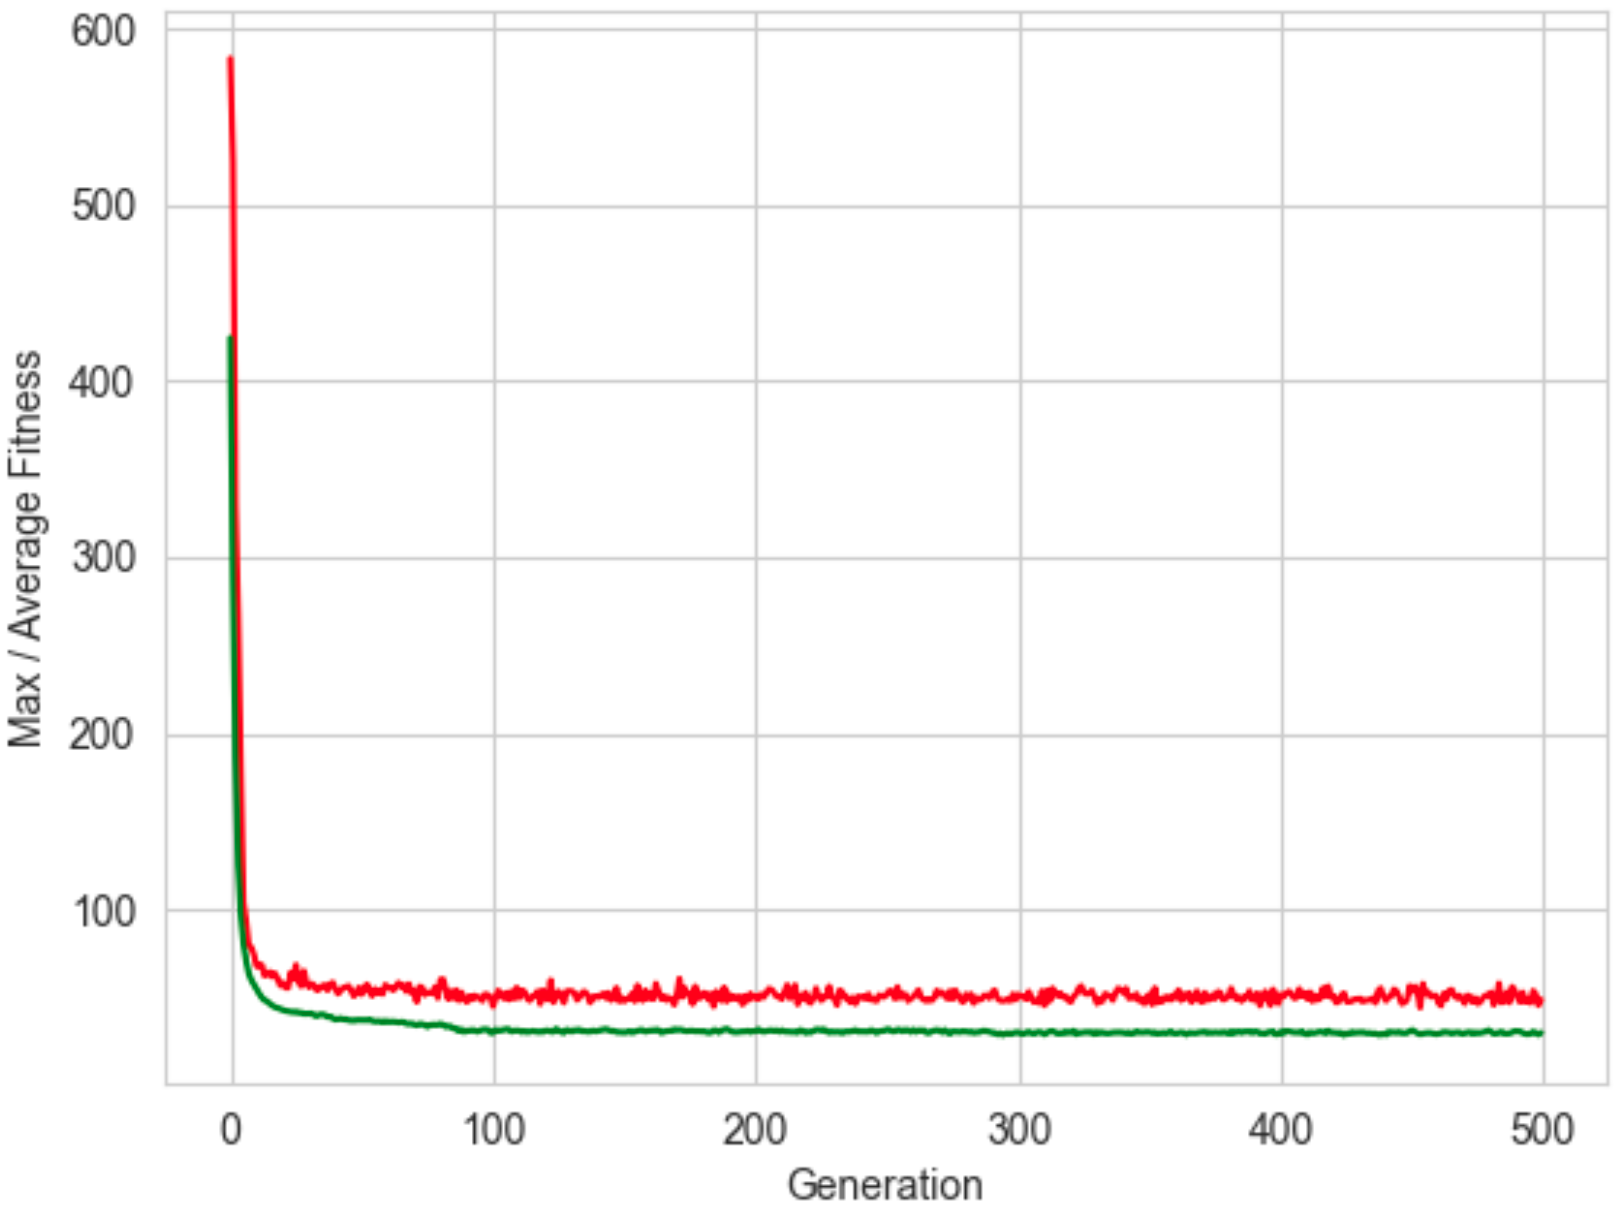
\includegraphics[width=\linewidth]{img_7}
  \caption{Max and Average Fitness over Generation}
  \Description{}
\end{figure}

%%
%% The acknowledgments section is defined using the "acks" environment
%% (and NOT an unnumbered section). This ensures the proper
%% identification of the section in the article metadata, and the
%% consistent spelling of the heading.

%%
%% The next two lines define the bibliography style to be used, and
%% the bibliography file.
\bibliographystyle{ACM-Reference-Format}
\bibliography{socio}
%%
%% If your work has an appendix, this is the place to put it.
\appendix


\end{document}
\endinput
%%
%% End of file `sample-sigconf.tex'.
